\documentclass[12pt]{report}
\usepackage[utf8]{inputenc}
\usepackage[demo]{graphicx}
\usepackage{blindtext}
\usepackage{subfig}
\usepackage{caption}

\begin{document}

\begin{figure}[h!]
    \centering
    \begin{subfigure}{0.5\textwidth}
      \centering
      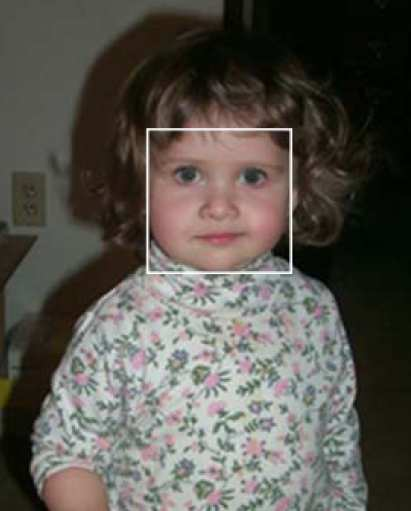
\includegraphics{../img/17_1.png}
      \caption{Face Detection}
      \label{fig:sub1}
    \end{subfigure}%
    \begin{subfigure}{0.5\textwidth}
      \centering
      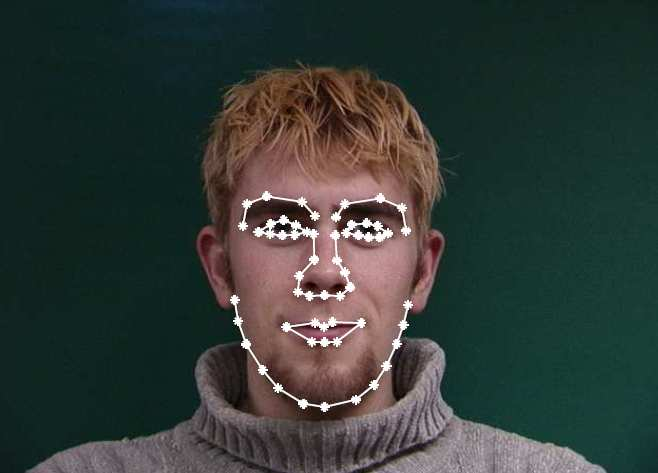
\includegraphics{../img/17_2.png}
      \caption{Face Alignment}
      \label{fig:sub2}
    \end{subfigure}
    \caption{Detection Vs. Alignment}
    \label{fig:test}
\end{figure}

\begin{figure}[h!]
    \centering
  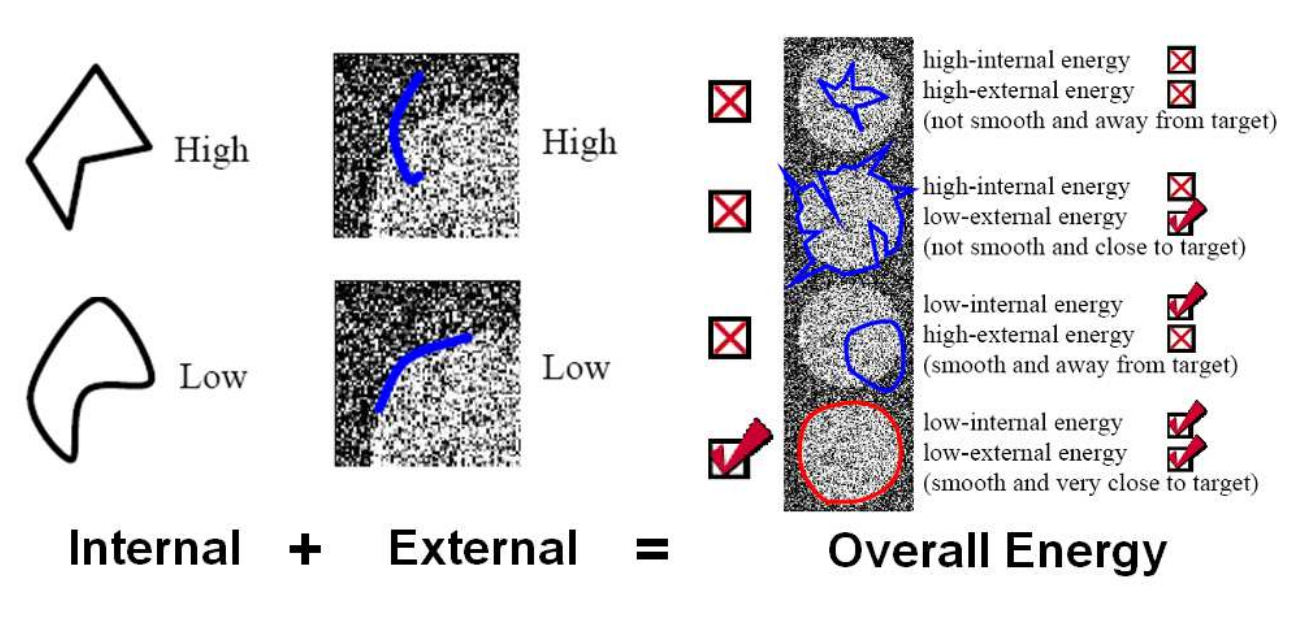
\includegraphics[width=\textwidth]{../img/18_1.png}     
      \caption{Energy function and curve fitting}
    \label{fig:face}
\end{figure}

\paragraph{}
It’s worth pointing out that sometimes the energy function is not explicitly given, instead it’s implicitly defined in the searching scheme, for example, in Active Shape Model.

\section{Feature Extraction}
“Feature extraction converts pixel data into a higher-level representation of shape, motion, color, texture, and spatial configuration of the face or its components. The extracted representation is used for subsequent classification. Feature extraction generally reduces the dimensionality of the input space. The reduction procedure should (ideally) retain essential information possessing high discrimination power and high stability”. In the face recognition area, various features have been used.

The coefficients of Eigenface can be used as features and recently, an extension of Eigenface defines Tensorface which has shown a promising choice of feature. Active Appearance Model  decomposes the facial image into “shape” and “texture”. The shape vector which is coded using ASM describes the contour of the facial components, whereas
the texture vector gives the “shape-free” facial texture. Matsuno et al.  extract features using a two-dimensional mesh, called Potential Net. All the above-mentioned methods are considered as holistic features, because they are related to the overall structure of the image. There is another kind of features called local features, each of which focuses only on a small region. The most straightforward idea may be to directly use image sub-windows as local features: for example, in \cite{15} Colmenarez \textit{ et al}. use nine sub-windows located around the facial components. Wavelet filters have been used too, the most popular of which is the Gabor filter which has been shown \cite{22} \cite{37} to be a reasonable model of visual processing in primary visual cortex. Yin and Wei use topographic primitive features to represent faces \cite{103}. In \cite{104}, instead of defining features ahead of time, Yu and Bhanu use a evolutionary algorithm to generate features automatically. For video-based FER, the dynamic of expression can also serve as features. \cite{44} proposes Geometric Deformation Feature which represents the geometrical displacement of certain selected landmark nodes. In \cite{1}, Aleksic and Katsaggelos use Facial Animation Parameters which are based on Active Shape Model.
\par In this section, we'll briefly introduce some of these feature extraction methods
\par
\section {Tensorface}
Tensorface \cite{90} is a multilinear extension of Eigenface. Instead of representing the face image using a linear equation.
\begin{equation}
x=\overline{x}+\sum_{i}a_i x_i
\end{equation}
It models the face by a multilinear system which is equivalent to
\begin{equation}
x=\overline{x}+\sum_{i_1}...\sum_{i_1}a_{i_N}...a_{i_N} x_{i_1}..._{i_N}
\end{equation}
\par 
Compared to Eigenface which ignores the label of images, Tensorface analyzes a face ensemble with respect to its underlying factors(labels): for example, identities, views, and illuminations. The "principal components" in this multilinear system are referred to as Tensorfaces which are shown in Fig.2.9. The Tensorface coefficients a$_{i_k}$ can be used as features in a recognition task, and because the original image can be reproduced using 2.26, Tensorface coefficients can also be used for image synthesis where we first generate a set of coefficients, then use them to synthesize images.

\par
Since Tensorface is shown to be a promising method in face recognition, some improvements have been proposed. \cite{92} proposes Multilinear Independent Component Analysis where they try to find the independent directions of variation. In \cite{76} Shashua et al. introduce Non-Negative Tensor Factorization which is a generalization of Non-negative Matrix Factorization.
\par 
\begin{figure}
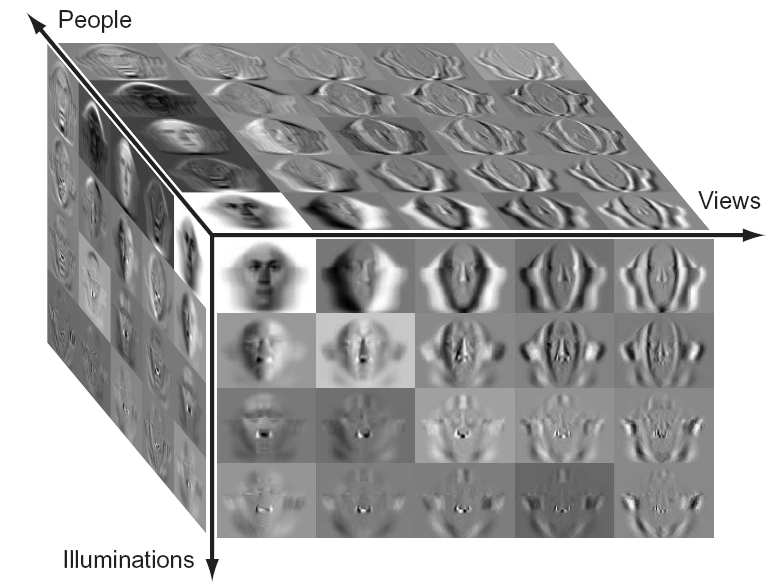
\includegraphics[width=\textwidth]{../img/20_1.png}
\caption{A partial visualization of TensorFaces bases for an ensemble of 2,700 facial images spanning 75 people, each imaged under 6 viewing and 6 illumination conditions \cite{92}}
\label{Fig 2.9}
\end{figure}
\section{Potential Net}
\par 
Matsuno \textit{et al}. \cite{61} \cite{41} propose Potential Net to extract facial features. As shown in Fig.2.10, Potential Net is a two dimensional mesh of which nodes are connected to their four neighbors with springs, while the most exterior nodes are fixed to the frame of the Net. Similar to curve fitting, Potential Net considers two forces: each node in the mesh is driven

\end{document}